%-----Chapter 2: Simulation-------%
% -  -  -  -  -  -  -  -  -  -  -  -  -  -  -  -  -  -  -  -  -  -  -  -  -  -  -  -  -  -  -  -  -  -  -  -  -  -  -  -  -  -  -  -  -  -  -  -  -  -  -  -  - %
\chapter{Simulation}

One main aspect of this group work among the design of a Kalman filter was the construction of a graphical environment for our work. So we decided to implement a simulation of a Nao soccer match in MATLAB. Therefore we made four independent modules which build the framework for the simulation. The four parts contain functions concerning the dynamics of the robots and ball, the measurements and the plots. Since these parts are constructed in a modular fashion, we can change one module without influencing the others. All functions mentioned below will build the core of a simple random simulation of a RoboCup soccer match. The simulation is called random because the input paramters of the robots, i.e. their velocity and their change of angular direction, are chosen randomly. The script {\fontfamily{pcr}\selectfont RoboCupSim.m} is essentially a finite loop with the described functions in it. Every step the in loop generates a new frame of our simulation. Most of the global variables are defined in {\fontfamily{pcr}\selectfont RoboCupSim.m} such as the dimensions of a real RoboCup playing field or all noise-relevant parameters. Also variables which cannot be initialized in a function, such as the covariance matrices for the Kalman filters, which will be discussed later, are defined in this script. The pseudocode below shows the general structure of our simulation framework and emphasizes the modularity of our code

% Pseudocode
\begin{verbatim}
      General settings
      Initialize Field Parameters
      Initialize Noise Parameters
      Initialize Robot and Ball Parameters

      Begin Loop
	
            Robot dynamics
            Ball dynamics
            Robot measurement
            Ball measurement
            Robot filtering
            Ball filtering
            Plot environment and objects
            // Debugging tool
	
      End Loop
\end{verbatim}

This chapter focuses on the implementation of the plot functions and the computation functions. The filter task of the simulation will be discussed in chapter 4.
The section about plots is mainly a documentation of the draw functions for the field and objects we made to illustrate the simulation, while the section about robots and ball also covers the mathematical background.

% -  -  -  -  -  -  -  -  -  -  -  -  -  -  -  -  -  -  -  -  -  -  -  -  -  -  -  -  -  -  -  -  -  -  -  -  -  -  -  -  -  -  -  -  -  -  -  -  -  -  -  -  - %
\section{Plots}
Plotting a step in the simulation can be divided essentially in two parts. One part contain the static part, such as the field or goals and the other part all dynamic objects, e.g. the robots and the ball.

\subsection*{Plot of the field - \texttt{plot\_env()} }
All graphical features concerning the playing field are implemented by the function \texttt{ plot\_env()}. It is subdivided in two functions, which draw the field and, as a neat add on, the scorecounter seperately. The size of the field and of the goals we took from the RoboCup Nao Rule Book 2011 and are defined in the global Struct \texttt{Field}.
\begin{lstlisting}
global Field;
    Field.width = 6; %[m]
    Field.height = 4; %[m]
    Field.penaltyAreaWidth = 0.6; %[m]
    Field.penaltyAreaHeight = 2.2; %[m]
    Field.goalHeight = 1.4; %[m]
    Field.goalWidth = 0.02; %[m]
    Field.centerCircleRadius = 0.6; %[m]
    Field.pointRadius = 0.05; %[m]
    Field.penaltyPointLocation = 1.8; %[m]
\end{lstlisting}
\vspace{+10pt}

To draw the field we mostly use built-in MATLAB commands such as \texttt{ rectangle()} or \texttt{ line()}. Only for drawing circles we made the function
	\[ \textnormal{\texttt{draw\_circle(x,y,r,color,isFilled)}}
	\]
where
\begin{description}
	\item[\texttt{x,y}] is position of the origin of the circle
	\item[\texttt{r}] is radius of the circle
	\item[\texttt{color}] is a string for the color of the circle, e.g. \texttt{'k','r'}
	\item[\texttt{isFilled}] is a boolean variable,\\
	\texttt{= 0} only the contour of the circle will be plotted in \texttt{color},\\
	\texttt{= 1} the circle will be plotted filled in \texttt{color}
\end{description}

The playing field after the execution of \texttt{ plot\_env()} is displayed in figure \ref{Playing_field}.

\begin{figure}[h]
	\centering
    	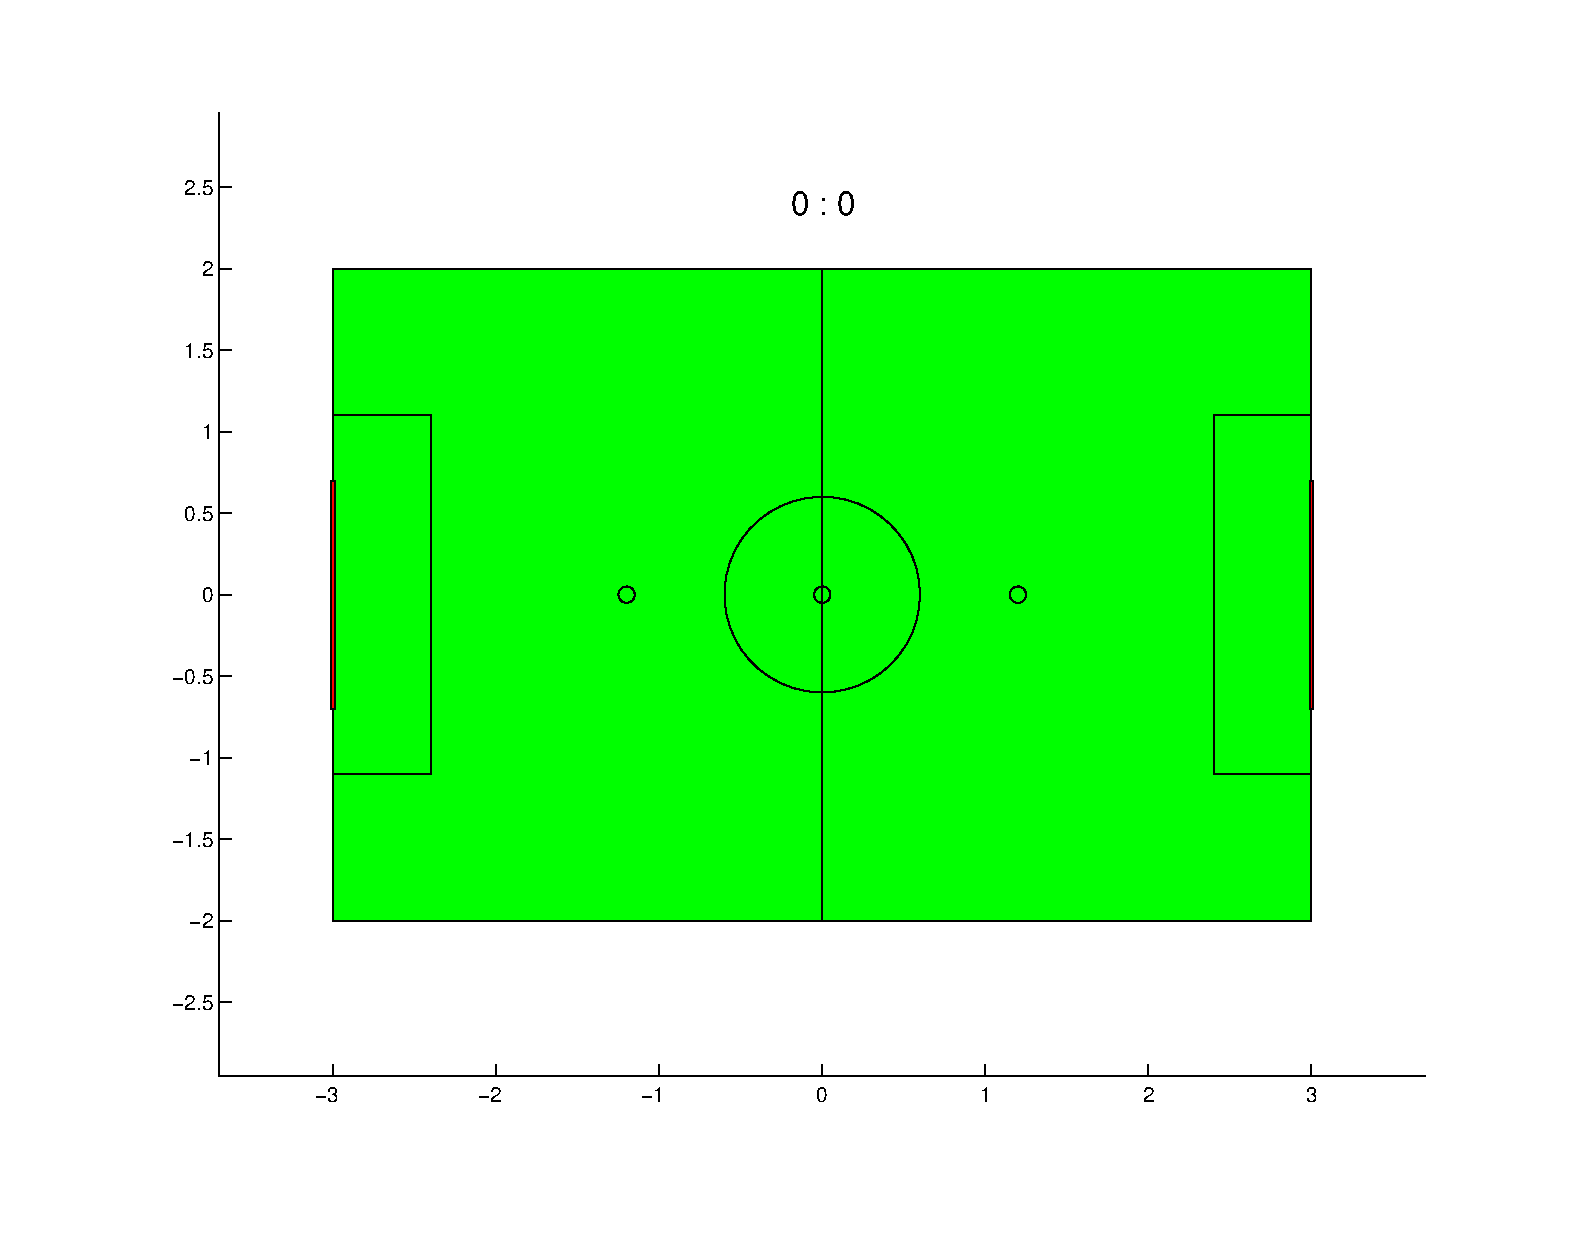
\includegraphics[width=12cm]{./2_Simulation/playing_field}
  	\caption{Playing field with \texttt{plot\_env()}.}
  	\label{Playing_field}
\end{figure}
\pagebreak[4]

\subsection*{Plot of the robots and ball - \texttt{plot\_objects(Robot,Ball,style)} }
To plot robots and ball we made the function
	\[ \textnormal{\texttt{plot\_objects(Robot,Ball,style)}}
	\]
where
\begin{description}
	\item[\texttt{Robot}] is a struct of robotstructs as described in section \ref{Robotsection}
	\item[\texttt{Ball}] is a ballstruct as described in section \ref{Ballsection}
	\item[\texttt{style}] is a string defining the rooter shape, which contain an arbitrary number and order of following characters\\
		\texttt{'0'} Draws circles in true size \\
		\texttt{'@'} Same as above, but filled \\
		\texttt{'-'} Includes the direction indicator\\
		\texttt{'+'} Draws crosses\\
		\texttt{'\#'} Enumerate Robots\\
		\texttt{'V'} Sight of view for blue team only\\
		\texttt{'Va'} Sight of view all robots \vspace{0.2cm} \\ 
		and one of the following character to specify the robot color\\
		\texttt{'t'} Team specific colors (blue and magenta) \\
		\texttt{'r','k','b',$\ldots$} other MATLAB colors
\end{description}
This different shape styles allows to display different robots, e.g. the real and the filtered robots, in a clear manner. 
Figure \ref{Playing_field_robots} shows the playing filed after initialization and execution of \texttt{plot\_env()} and \texttt{plot\_objects(Robot,Ball,'@-t')}. Where \texttt{Robot} and \texttt{Ball} are the standard initialization structs as described in Section \ref{Robotsection} and \ref{Ballsection}.

\begin{figure}[h]
	\centering
    	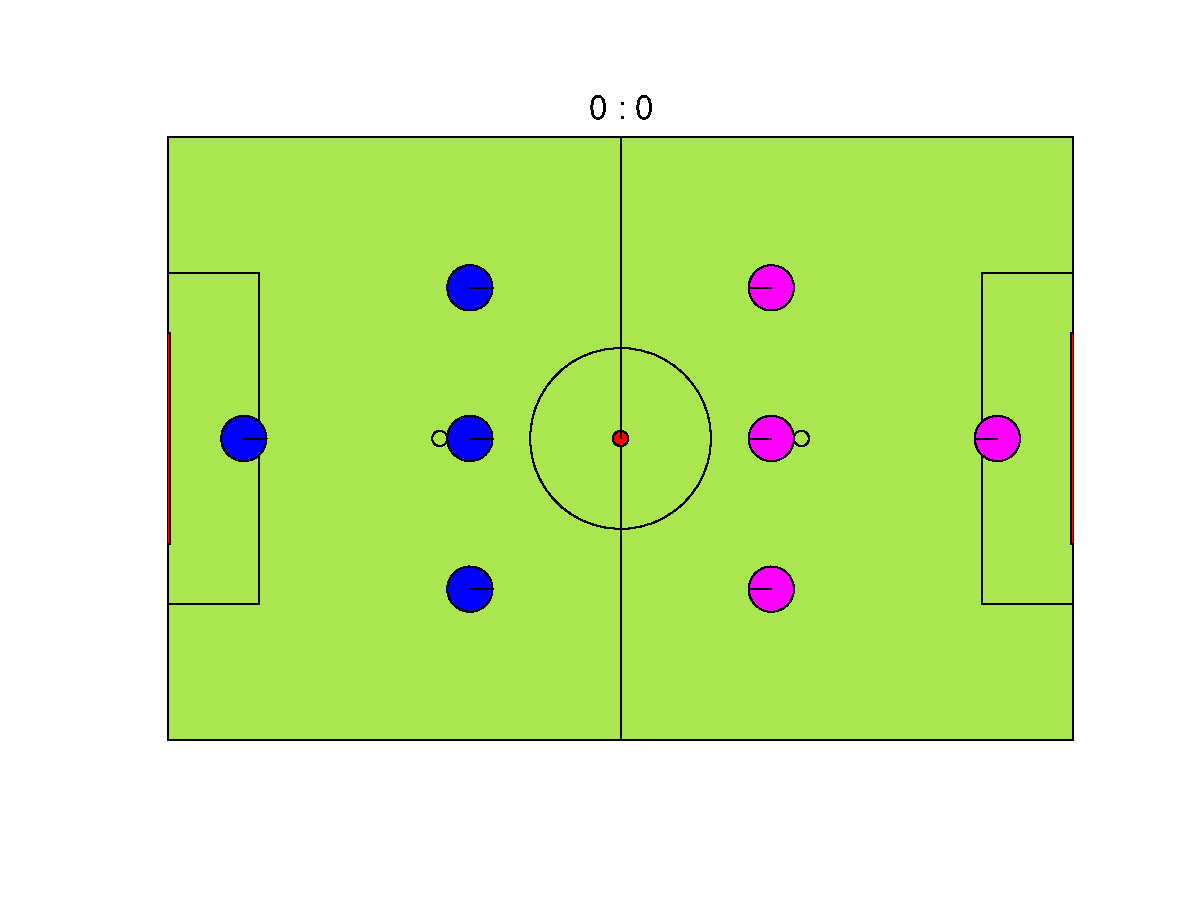
\includegraphics[width=12cm]{./2_Simulation/playing_field_robots}
  	\caption{Playing field after initialization and \texttt{plot\_objects(Robot,Ball,'@-t')}.}
  	\label{Playing_field_robots}
\end{figure}


% -  -  -  -  -  -  -  -  -  -  -  -  -  -  -  -  -  -  -  -  -  -  -  -  -  -  -  -  -  -  -  -  -  -  -  -  -  -  -  -  -  -  -  -  -  -  -  -  -  -  -  -  - %
\section{Robots} \label{Robotsection}

Maybe the most important part of the simulation is the adequate depiction and behaviour of all eight robots. The task can be separated in two components: After the robots are initialized, their new positions on the field, according to their motion equations, are computed.
%The latter task is split in three components: I and in the end we are adding measurement noise for our filtering task.

\subsection*{Initialization}
The initialization of the robots is quite simple. The function \texttt{ robot\_standard\_init()} creates a struct of eight structs with the essential informations for every robot, i.e. its horizontal and vertical position, its direction and its team affiliation. Following tabular depicts the structure of such a struct.

\begin{center}
	\begin{tabular}{| l | l | c | l |} \hline
		\texttt{Robot(1)} & \texttt{Robot(2)} & $\cdots$ & \texttt{Robot(8)}  \\ \hline
		\texttt{.color} & \texttt{.color} & &\texttt{.color} \\
		\texttt{.x} & \texttt{.x} & & \texttt{.x} \\
		\texttt{.y} & \texttt{.y} & & \texttt{.y} \\
		\texttt{.dir} & \texttt{.dir} & & \texttt{.dir}\\ \hline
	\end{tabular}
\end{center}
 
Furthermore the initialization function defines some robot specific parameters in the global struct \texttt{RobotParam}. This are characteristics such as the robot's radius or its maximum possible angular change for one time step. In a latter stage of development we dropped the simplification of a global eye and assumed that a location of a robot's position is only possible if it is in the sight of view of at least one other robot. So additionally parameters of sight distance as well as its angle of sight are set in the initialization function. The MATLAB code below shows our assumptions for these parameters
\begin{lstlisting}
    global RobotParam dt;
    RobotParam.radius = 0.15; %[m]
    RobotParam.velocity = 0.1 * dt; %[m/step]
    RobotParam.changeOfDir = 0.1 * 2*pi * dt; %[rad/step]
    RobotParam.sightDistance = 2.5; %[m]
    RobotParam.sightAngle = pi./6; %[rad]
\end{lstlisting}
  
\subsection*{Dynamics of the robots - Mathematical model}
%Once initialized we use the functions \texttt{ dummy\_step(Robot).m} and \texttt{ robot\_step(Robot,Ball).m} respectively to compute the attributes of all robots for every timestep. The key issue of both functions however is the recalculation of the position, i.e. the motion of the robots
To compute the next step of the robots we used the following simple non-linear discrete time motion equations
\begin{eqnarray}
	x_{i_{k+1}} &=& x_{i_{k}} + v_{i_{k}} \cos(\varphi_{i_{k}}) \Delta t 	\label{robot_motion_first} \\
	y_{i_{k+1}} &=& y_{i_{k}} + v_{i_{k}} \sin(\varphi_{i_{k}}) \Delta t \\
	\varphi_{i_{k+1}} &=& \varphi_{i_{k}} + d\omega_{i_k} \Delta t
	\label{robot_motion_last}
\end{eqnarray}
with the boundary conditions, that the robots have to be on the playing field and can't covering the same disk as another robot:
	\[ (x_{i_{k}},y_{i_{k}}) \in [-3+r_r,3-r_r]\times[-2+r_r,2-r_r] \quad \forall k, \forall i\in \{1,2,\ldots,8 \}
	\]
	\[ \sqrt{(x_{i_{k}}-x_{j_{k}})^2 + (y_{i_{k}}-y_{j_{k}})^2} =: d_{ij} \geq 2r_r \quad \forall k, \forall i, \forall j\neq i
	\]
Where $(x_i,y_i)$ is the position and $\varphi_i$ the direction of robot $i$ and $r_r$ the radius of a robot. The velocity $v_i$ and the change of direction $d\omega_i$ are inputs to the system.

%\lstinputlisting[firstline=20, lastline=27]{../Simulation/Merge/dummy_step.m}

%Later the non-linearity of these equations will make it necessary that we use an extended Kalman filter instead of a simple linear one. The addition of process noise and the collision handling of robots also happen in these functions. The process noise we use for our model is always white Gaussian noise with seperate covariances for the positions and the directions. 
\subparagraph{Random Collision Roboter} To satisfy the boundary conditions we first used robots which rebounce when they collide into the sidelines and into each other. If they hit each other they swap direction 
%. In \texttt{ dummy\_step(Robot).m} we used a very simple model, assuming that if two robots collide, their directions swap such that they do not run into each other
%\lstinputlisting[firstline=52, lastline=54]{../Simulation/Merge/dummy_step.m}
and if they touch a sideline, they reflect after the law of reflection 
\[ \Theta_{\textnormal{in}} = \Theta_{\textnormal{out}}.
\]
Those dynamics are implemented in \texttt{robot\_rand\_step(Robot)} with a random inputs $d\omega_{i_k} \sim \mathcal{N}(0,0.2\pi \cdot dt)$ and constant velocities $v_{i_k} = v = 0.1 m/s$.\\

But this solution was not optimal for two reasons: First we had the problem that there was a bug which made it possible that two robots became wedged together and their further behaviour was messed up after they had contact. The second problem was, that our Kalman filter didn't work properly since the swapping of directions is a rapid change in states, which cannot be handled by a normal Kalman filter. 

\subparagraph{Random Potential Roboter} 
The function \texttt{ robot\_randpot\_step(Robot,Ball)} eliminates both issues because it doesn't use collision detection but collision avoidance. If the distance of two robots falls below a given radius $r_a$, we assign a potential to both robots. The effect is now similar to this of a positive charge in an electrostatic field: The closer two robots are, the bigger is their mutual repulsion. The force in a electric field is given by
	\[ F = m\ddot{x} = C \frac{1}{x^2}.
	\]
Integration results in
	\[ \dot{x} = \frac{dx}{dt} = \tilde{C} \frac{1}{x}.\]
Or the same described in vector notation:
	\[	\vec{F} = C \frac{\vec{r}}{|\vec{r}|^3} \qquad \Rightarrow \qquad \dot{\vec{r}} = \frac{d \vec{r}}{dt} = %
			\tilde{C} \frac{\vec{r}}{|\vec{r}|^2} %
	\]
As you can see in the code below, we use the same \(r^{-2}\)-relation for the repulsing force as it is known from the analysis of electrostatic fields
\begin{lstlisting}
        for j=1:8
           % Distance between robot i and j
           r = sqrt((Robot(j).x-Robot(i).x).^2+(Robot(j).y-Robot(i).y).^2);
            
           % Potential function to compute repulsion between robots.
           if ( i~=j && (r <= ra) )
               dx = dx + C./r.^3*(Robot(i).x-Robot(j).x);
               dy = dy + C./r.^3*(Robot(i).y-Robot(j).y);
           end
        end
\end{lstlisting}

A related potential is also assigned to the sideline, if a robot is under a given distance $r_f$ to it. With those potentials, the change of directions is now continuous, which makes tracking possible for our Kalman filter. Additionally to the collision avoidance the robots are attracted to the ball if it's near them, like it had a negative charge. This leads to some more ball contacts than before.

\textcolor{red}{evtl. Bild Potential}


%In the simulation we used a radius 

% -  -  -  -  -  -  -  -  -  -  -  -  -  -  -  -  -  -  -  -  -  -  -  -  -  -  -  -  -  -  -  -  -  -  -  -  -  -  -  -  -  -  -  -  -  -  -  -  -  -  -  -  - %
\section{Ball} \label{Ballsection}

The treatment of the ball is quite similar to that of the robots. The ball object is also represented by a struct containing its horizontal and vertical position, its direction and different than the robot also the velocity.
\begin{center}
	\begin{tabular}{| l |} \hline
		Ball \\ \hline
		.x \\
		.y \\
		.dir \\
		.velocity \\ \hline
	\end{tabular}
\end{center}
 These parameters are set by executing \texttt{ ball\_init()}. This function also defines the ball's radius, its initial velocity and the friction towards the ground in the global struct \texttt{BallParam}. In our simulation we used following parameters for the ball
\begin{lstlisting}
    global BallParam dt;
    BallParam.radius = 0.05; %[m]
    BallParam.velocity = 0.4 *dt; %[m/step]
    BallParam.friction = 0.995;
\end{lstlisting}
 
\subsection*{Dynamics of the ball - Mathematical model}
%The function \texttt{ ball\_step(Ball,Robot).m} does, like the equivalent function for the robots, the computations of the ball's next position and direction on the field. These parameters however do not only depend on the ball's dynamics but also whether it collides with one of the robots. The following MATLAB code shows the algorithm for this collision detection

%\lstinputlisting[firstline=40, lastline=51]{../Simulation/Merge/ball_step.m}
The dynamics of the ball are fairly analog to those of the robots. Only that the velocity is no longer an input but now a state of the system and there is some friction between the ball and ground. 
The the non-linear motion equation for the ball are therefore
\begin{eqnarray}
	x_{{k+1}} &=& x_{k} + v_{k} \cos(\varphi_{k}) \Delta t	\label{ball_motion_first} \\
	y_{{k+1}} &=& y_{k} + v_{k} \sin(\varphi_{k}) \Delta t \\
	\varphi_{{k+1}} &=& \varphi_{k}\\
	v_{{k+1}} &=& \varrho \cdot v_{k}
	\label{ball_motion_last}
\end{eqnarray}
With the boundary conditions, that the ball has to stay on the playing field and can't be under a robot
	\[ (x_{k},y_{k}) \in [-3+r_b,3-r_b]\times[-2+r_b,2-r_b] \quad \forall k, 
	\]
	\[ \sqrt{(x_{k}-x_{_i{k}})^2 + (y_{k}-y_{j_{k}})^2} =: d_{bi} \geq r_r + r_b \quad \forall k, \forall i
	\]
To satisfy these conditions, we used for the sidelines again the law of reflection.  And if the ball collides with one of the robots, it regains its initial velocity and bounces away, perpendicular to the robot's position. Like the robot had kicked the ball. These dynamics are implemented in the function \texttt{ball\_step(Ball)}.

% -  -  -  -  -  -  -  -  -  -  -  -  -  -  -  -  -  -  -  -  -  -  -  -  -  -  -  -  -  -  -  -  -  -  -  -  -  -  -  -  -  -  -  -  -  -  -  -  -  -  -  -  - %
\section{Noise}
Up to this point we computed the behavior of an ideal robot and ideal ball. Since our goal is to filter out the uncertainty of motion of the robot parameters, we artifically have to add some measurement noise which we can filter later on. %The functions \texttt{ dummy\_measure(Robot)} and \texttt{ robot\_measure(Robot)} are implemented for that purpose.
Also we added some process noise to the dynamics of robots and ball, which can't be filtered.
Hence the motion equations get extended as followed
\begin{eqnarray*}
	x_{k+1} &=& {f}({x}_k,{u}_k) + {w}_k \\
	{z}_{k} &=& {x}_k + v_k
\end{eqnarray*}
where $x$ is the state, $z$ the output, $f()$ the nonlinear system of equations in (\ref{robot_motion_first}-\ref{robot_motion_last}) or (\ref{ball_motion_first}-\ref{ball_motion_last}), $w$ the process noise vector and $v$ the measurement noise vector.\\

The process noise $w$ we added in the specific step functions for robots and ball as white Gaussian noise.
The measurement noise is white Gaussian, too. But additionally we made two different implementations, which determine if there is a measurement at all or the corresponding parameters are just dropped.

\subparagraph{Random measurement}
The function \texttt{ robot\_random\_measure(Robot)} simply adds white Gaussian noise to the position and the direction of every robot. Additionally with a certain possibility there is no measurement at all.  \texttt{ball\_random\_measure(ball)} does the same for the ball. What we are assuming with this model is, that there is some global eye available which measures the position and direction of every robot with some given resolution. But this scenario is not realistic in a RoboCup soccer match, because only the robots themselves can gain visual information.

\subparagraph{Sight of view measurement} The functions \texttt{robot\_sight\_of\_view\_measure(Robot)} for the robots and \texttt{ball\_sight\_of\_view\_measure(Ball)} for the ball solve this problem. According to a sight of view, a measurement of a robot is only available if it stands in front of a characteristic point on the field or if it is within the distance of sight of another robot. Note that a robot only locates other robots if it is aware of its own position and that we get information from only one team, which will be the case for official RoboCup matches.

%After this computational part, the robots are added to the graphical environment by using the function
%\texttt{ plot\_robot(Robot,Ball,style).m}. It provides several features such as the coloration, the shape and the label of the robots on the field. A sample output on the graphical interface after several timesteps is shown in figure \ref{Plot_robots} below.

%\begin{figure}[htbp]
%	\centering
%    	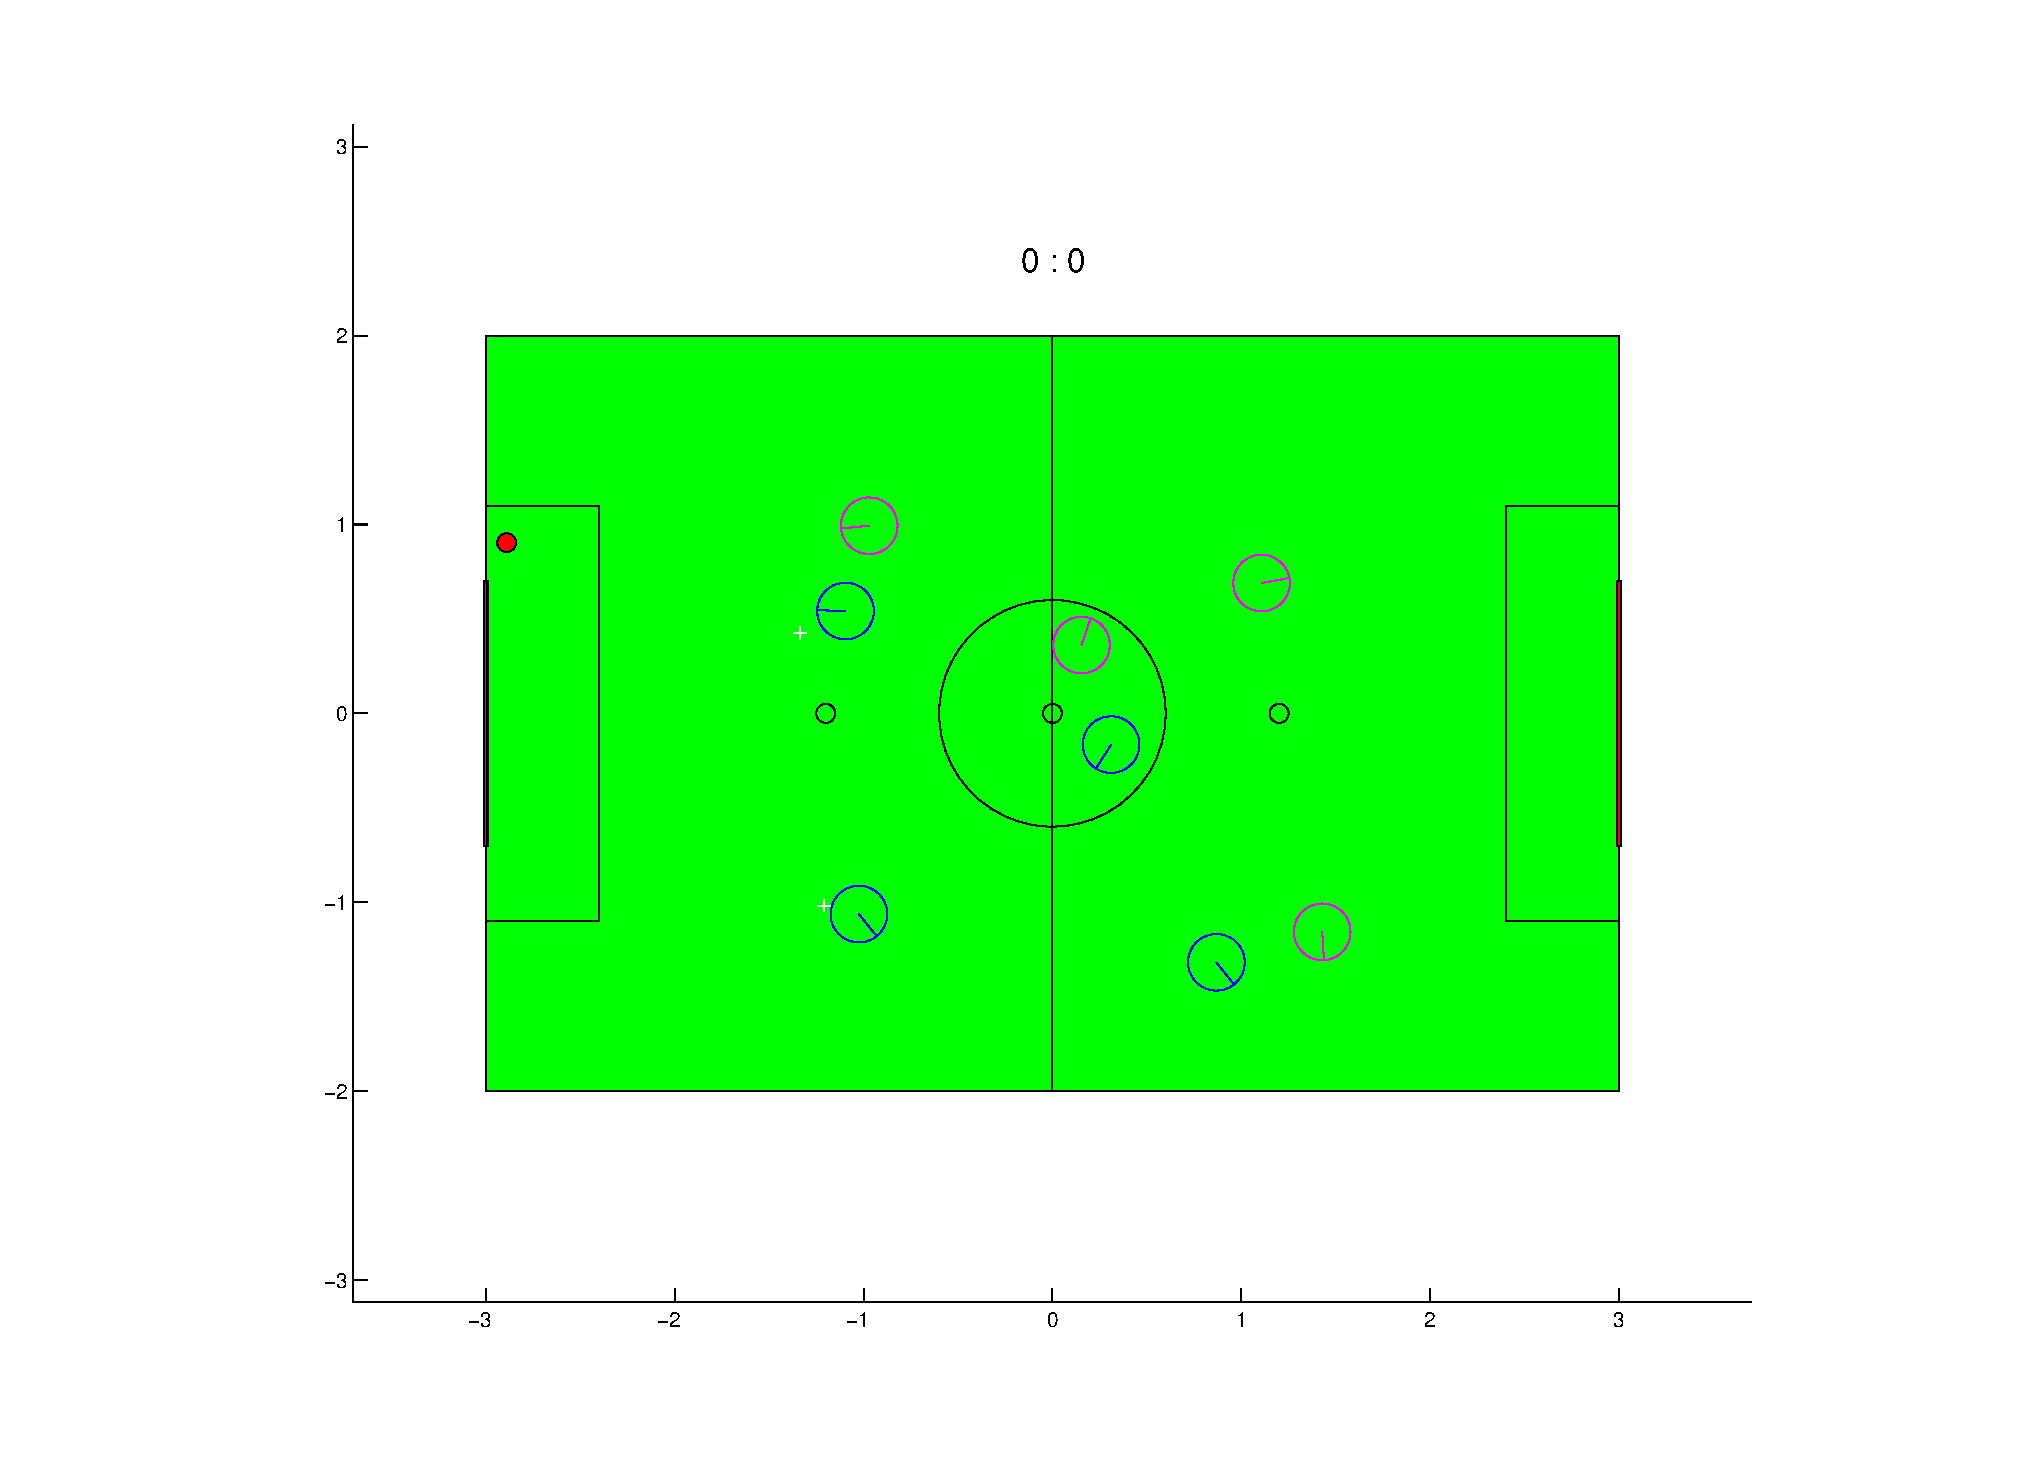
\includegraphics[width=12cm]{./2_Simulation/plot_robots}
%  	\caption{Capture of a regular simulation frame.}
%  	\label{Plot_robots}
%\end{figure}

%Note that measurements (white crosses) are not available for most robots (blue and magenta circles).



%Since the ball too is a subject of measurement, we also needed a measurement function for this object. \texttt{ ball\_measure(Ball).m} adds measurement noise or, as the case may be, drops the measurement completely. Again, a measurement is only available if it is in the sight of view of at least one blue robot that knows its own position. For more than one measurement the mean value of all measurements is taken. After all computations are done, the ball is drawn on the field, together with the robots, with the function \texttt{ plot\_robot(Robot,Ball,style).m}. All features of this function like coloration and drawing of different shapes are also available for the ball.

